\documentclass[14pt]{extarticle}
\usepackage{extsizes}

\usepackage[T2A]{fontenc}

\usepackage[utf8]{inputenc}
\usepackage[russian]{babel}

\usepackage{geometry}
\geometry{a4paper, left=30mm, right=15mm, vmargin=20mm}

\setlength{\parindent}{1.25cm}
\usepackage{indentfirst}

\usepackage{setspace}
\onehalfspacing

\usepackage{graphicx}
\usepackage{ulem}

\begin{document}

\begin{titlepage}
\newgeometry{a4paper, left=20mm, right=20mm, vmargin=20mm}

\noindent
\begin{minipage}{0.15\textwidth}
    
\includegraphics[width=\textwidth]{resources/bmstu-logo.png}
\end{minipage}
\noindent
\begin{minipage}{0.80\textwidth}
    \bfseries\small\centering
    Министерство науки и высшего образования Российской~Федерации
    \\
    Федеральное государственное бюджетное образовательное учреждение высшего
    образования
    \\
    <<Московский государственный технический университет имени Н.\,Э.~Баумана
    \\
    (национальный исследовательский университет)>>
    \\
    (МГТУ им. Н.\,Э.~Баумана)
\end{minipage}

\bigskip
\noindent
\rule{\textwidth}{3pt}

\noindent
ФАКУЛЬТЕТ
\uline{<<Информатика и системы управления>> \hfill}

\noindent
КАФЕДРА
\uline{<<Программное обеспечение ЭВМ и информационные технологии>> \hfill}

\begin{center}
    \bfseries\large
    Отчёт по лабораторной работе №\,1
    \\
    по дисциплине <<Операционные системы>>
\end{center}

\noindent
\textbf{Тема}
\uline{Прерывание таймера в системах разделения времени \hfill}

\noindent
\textbf{Студент}
\uline{Кириченко~С.\,П. \hfill}

\noindent
\textbf{Группа}
\uline{ИУ7-51Б \hfill}

\noindent
\textbf{Оценка (баллы)}
\uline{\hfill}

\noindent
\textbf{Преподаватель}
\uline{Рязанова Н.\,Ю. \hfill}

\begin{center}
    \vfill
    Москва~---~\the\year~г.
\end{center}

\restoregeometry
\end{titlepage}

\setcounter{page}{2}

\section{Функции системного таймера}

\subsection{В операционных системах семейства Windows}

\paragraph{По тику}
\begin{itemize}
    \item инкремент счетчика системного времени;
    \item декремент кванта текущего потока;
    \item декремент счетчиков отложенных задач.
\end{itemize}

\paragraph{По главному тику}
\begin{itemize}
    \item инициализация диспетчера настройки баланса путем сбрасывания объекта
        <<событие>>, на котором он ожидает.
\end{itemize}

\paragraph{По кванту}
\begin{itemize}
    \item Инициация диспетчеризации потоков~--- постановка соответствующего
        объекта в очередь DPC.
\end{itemize}

\subsection{В операционных системах семейства Unix}

\paragraph{По тику}
\begin{itemize}
    \item инкремент счетчика времени с момента запуска системы (в системе
        SVR4~--- переменной \texttt{lbolt});
    \item инкремент счетчика реального времени;
    \item инкремент часов и других таймеров системы;
    \item декремент счетчиков времени и при достижении счетчиками нулевого
        значение установка флага для обработчиков отложенных вызовов;
    \item инкремент счетчика процессорного времени, полученного процессором в
        режиме задачи и в режиме ядра.
\end{itemize}

\paragraph{По главному тику}
\begin{itemize}
    \item инициализация отложенного вызова функции планировщика;
    \item инициализация отложенного вызова процедуры \texttt{wakeup}, которая
        меняет состояние процесса с <<спящий>> на <<готовый к выполнению>>;
    \item пробуждение системных процессов, таких как \texttt{pagedaemon}.
    \item декремент счетчика времени, которое осталось до посылки одного из
        следующих сигналов:
    \begin{itemize}
        \item \texttt{SIGVTALRM}~--- сигнал, посылаемый процессу по истечении
            промежутка реального времени;
        \item \texttt{SIGPROF}~--- сигнал, посылаемый процессу по истечении
            времени, заданного в таймере профилирования;
        \item \texttt{SIGALRM}~--- сигнал, посылаемый процессу по истечении
            времени, заданного в <<виртуальном>> таймере.
    \end{itemize}
\end{itemize}

\paragraph{По кванту}
\begin{itemize}
    \item посылка сигнала \texttt{SIGXCPU} текущему процессу, если он превысил
        выделенную для него квоту процессорного времени.
\end{itemize}

\section{Пересчет динамических приоритетов}

Операционные системы семейств Unix и Windows являются системами разделения
времени с динамическими приоритетами и вытеснением. Динамические приоритеты
могут иметь только пользовательские процессы, другие процессы имеют
фиксированные приоритеты.

\subsection{В операционных системах семейства Windows}

Процессу при создании назначается приоритет. Относительно приоритета процесса
относительный приоритет назначается каждому потоку.

Планирование осуществляется на основании приоритетов потоков, готовых к
выполнению. Поток с более низким приоритетом вытесняется планировщиком, когда
поток с более высоким приоритетом становится готовым к выполнению. По истечению
кванта времени текущего потока, ресурс передается первому~--- самому
приоритетному~--- потоку в очереди готовых на выполнение.

Раз в секунду диспетчер настройки баланса сканирует очередь готовых потоков.
Если обнаружены потоки, ожидающие выполнения более 4 секунд, диспетчер
настройки баланса повышает их приоритет. Как только квант истекает, приоритет
потока снижается до базового приоритета. Если поток не был завершен за квант
времени или был вытеснен потоком с более высоким приоритетом, то после снижения
приоритета поток возвращается в очередь готовых потоков.

Чтобы минимизировать расход процессорного времени, диспетчер настройки баланса
сканирует лишь 16 готовых потоков. Кроме того, диспетчер повышает приоритет не
более чем у 10 потоков за один проход: обнаружив 10 потоков, приоритет которых
следует повысить, он прекращает сканирование. При следующем проходе
сканирование возобновляется с того места, где оно было прервано в прошлый раз.
Наличие 10 потоков, приоритет которых следует повысить, говорит о необычно
высокой загруженности системы.

В Windows предусмотренно 32 уровня приоритета:
\begin{itemize}
    \item приоритет 31~--- наивысший;
    \item от 16 до 31~--- процессы реального времени;
    \item от 0 до 15~--- динамические уровни;
    \item 0~--- зарезервирован для процесса обнуления страниц.	
\end{itemize}

Уровни приоритета потоков назначаются исходя из двух разных позиций: одной от
Windows API и другой от ядра Windows. Сначала Windows API систематизирует
процессы по классу приоритета, который им присваивается при создании:
\begin{itemize}
    \item Реального времени~--- Real-time (4)
    \item Высокий~--- High (3)
    \item Выше обычного~--- Above Normal (6)
    \item Обычный~--- Normal (2)
    \item Ниже обычного~--- Below Normal (5)
    \item Простоя~--- Idle (1)
\end{itemize}

Затем назначается относительный приоритет потоков в рамках процесса:
\begin{itemize}
    \item критичный по времени (time critical, 15);
    \item наивысший (highest, 2);
    \item выше обычного (above normal, 1);
    \item обычный (normal, 0);
    \item ниже обычного (below normal, -1);
    \item низший (lowest, -2);
    \item простой (idle, -15).
\end{itemize}

Соответствие между приоритетами Windows API и ядра системы приведено в таблице
\ref{tbl:priority}.

\begin{table}[h]
    \caption{Соответствие между приоритетами Windows API и ядра Windows}
    \centering
    \begin{tabular}{|l|p{45pt}|p{45pt}|p{45pt}|p{45pt}|p{45pt}|p{45pt}|}
        \hline
        & \textbf{real-time} & \textbf{high} & \textbf{above normal} & \textbf{normal} & \textbf{below normal} & \textbf{idle} \\
        \hline
        \textbf{time critical} & 31 & 15 & 15 & 15 & 15 & 15 \\
        \hline
        \textbf{highest} & 26 & 15 & 12 & 10 & 8 & 6 \\
        \hline
        \textbf{above normal} & 25 & 14 & 11 & 9 & 7 & 5 \\
        \hline
        \textbf{normal} & 24 & 13 & 10 & 8 & 6 & 4 \\
        \hline
        \textbf{below normal} & 23 & 12 & 9 & 7 & 5 & 3 \\
        \hline
        \textbf{lowest} & 22 & 11 & 8 & 6 & 4 & 2 \\
        \hline
        \textbf{idle} & 16 & 1 & 1 & 1 & 1 & 1 \\
        \hline
    \end{tabular}
    \label{tbl:priority}
\end{table}

Текущий приоритет потока в динамическом диапазоне может быть повышен
планировщиком вследствие следующих причин:
\begin{itemize}
    \item завершение операций ввода-вывода;
    \item повышение приоритета владельца блокировки;
    \item ввод из пользовательского интерфейса;
    \item длительное ожидание ресурса исполняющей системы;
    \item ожидание объекта ядра;
    \item готовый к выполнению поток не был запущен в течение длительного
        времени;
    \item повышение приоритета службой планировщика MMCSS.
\end{itemize}

\begin{table}[h]
    \caption{Рекомендуемые значения повышения приоритета}
    \centering
    \begin{tabular}{|p{100mm}|l|}
        \hline
        \textbf{Устройство} & \textbf{Приращение} \\
        \hline
        Диск, CD-ROM, параллельный порт, видео & 1 \\
        \hline
        Сеть, почтовый ящик, именованный канал, последовательный порт & 2 \\
        \hline
        Клавиатура, мышь & 6 \\
        \hline
        Звуковая плата & 8 \\
        \hline
    \end{tabular}
    \label{tab:io}
\end{table}

Текущий приоритет потока в динамическом диапазоне может быть понижен до
базового приоритета путем вычитания всех повышений.

\subsubsection{MMCSS}

Потоки, на которых выполняются различные мультимедийные приложения, должны
выполняться с минимальными задержками. В Windows эта задача решается путем
повышения приоритетов таких потоков драйвером MMCSS~--- MultiMedia Class
Scheduler Service. Приложения, которые реализуют воспроизведение мультимедиа,
указывают драйверу MMCSS задачу из списка:
\begin{enumerate}
    \item аудио;
    \item возможность использовать функции записи;
    \item воспроизведение звукового или видео контента;
    \item задачи администратора многооконного режима.
\end{enumerate}

Одно из наиболее важных свойств для планирования потоков~--- категория
планирования~--- первичный фактор определяющий приоритет потоков,
зарегистрированных в MMCSS. Различные категории планирования представленны в
таблице ниже.

\begin{table}[h!]
    \caption{Категории планирования.}
    \centering
    \begin{tabular}{|p{40mm}|p{30mm}|p{80mm}|}
        \hline
        \textbf{Категория} & \textbf{Приоритет} & \textbf{Описание} \\
        \hline
        High (Высокая) & 23-26 & Потоки профессионального аудио (Pro Audio),
        запущенные с приоритетом выше, чем у других потоков на системе, за
        исключением критических системных потоков \\
        \hline
        Medium (Средняя) & 16-22 & Потоки, являющиеся частью приложений первого
        плана, например Windows Media Player \\
        \hline
        Low (Низкая) & 8-15 & Все остальные потоки, не являющиеся частью
        предыдущих категорий \\
        \hline
        Exhausted (Исчерпавших потоков) & 1-7 & Потоки, исчерпавшие свою долю
        времени центрального процессора, выполнение которых продолжиться,
        только если не будут готовы к выполнению другие потоки с более высоким
        уровнем приоритета \\
        \hline
    \end{tabular}
    \label{tab:plan}
\end{table}

Функции MMCSS временно повышают приоритет потоков, зарегистрированных с MMCSS
до уровня, соответствующего их категориям планирования. Далее, их приоритет
снижается до уровня, соответствующего категории Exhausted, для того чтобы
другие потоки могли получить ресурс.

\subsubsection{IRQL}

Хотя контроллеры прерываний устанавливают приоритетность прерываний, Windows
устанавливает свою собственную схему приоритетности прерываний, известную как
уровни запросов прерываний (IRQL). В ядре IRQL-уровни представлены в виде
номеров от 0 до 31 (рисунок \ref{fig:irql}), где более высоким номерам
соответствуют прерывания с более высоким приоритетом.

\begin{figure}[h]
    \centering
    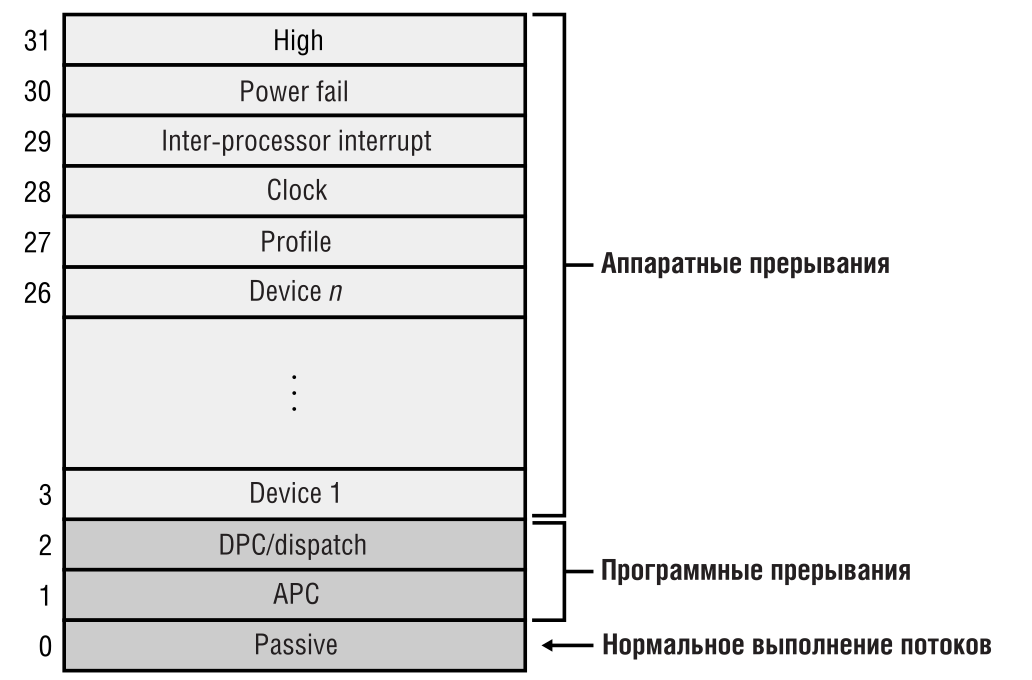
\includegraphics[width=0.90\linewidth]{resources/irql.png}
    \caption{Уровни запросов прерываний}
    \label{fig:irql}
\end{figure}

Прерывания обслуживаются в порядке их приоритета. При возникновении прерывания
с высоким приоритетом процессор сохраняет информацию о состоянии прерванного
потока и запускает связанные с прерывание диспетчер системных прерываний.

\subsection{Системы семейства Unix}

Планирование процессов в UNIX основано на приоритете процесса. Планировщик
всегда выбирает процесс с наивысшим приоритетом. Приоритеты планирования
изменяются с течением времени (динамически) системой в зависимости от
использования вычислительных ресурсов, времени ожидания запуска и текущего
состояния процесса. 

Традиционное ядро UNIX является строго невытесняющим, однако в современных
системах UNIX ядро является вытесняющим~--- то есть процесс в режиме ядра может
быть вытеснен более приоритетным процессом в режиме ядра. Ядро сделано
вытесняющим для того, чтобы система могла обслуживать процессы реального
времени, например видео и аудио.

Очередь процессов, готовых к выполнению, формируется согласно приоритетам и
принципу вытесняющего циклического планирования, то есть сначала выполняются
процессы с большим приоритетом, а процессы с одинаковым приоритетом выполняются
в течении кванта времени друг за другом циклически. В случае, если процесс с
более высоким приоритетом поступает в очередь процессов, готовых к выполнению,
планировщик вытесняет текущий процесс и предоставляет ресурс более
приоритетному процессу.

Приоритет процесса задается любым целым числом, которое лежит в диапазоне от 0
до 127 (чем меньше число, тем выше приоритет):
\begin{itemize}
    \item 0--49~--- зарезервированы для ядра (приоритеты ядра фиксированы);
    \item 50--127~--- прикладные (приоритеты прикладных задач могут изменяться
        во времени).
\end{itemize}

Изменение приоритета прикладных задач зависит от следующих факторов:
\begin{itemize}
    \item фактор <<любезности>>;
    \item последней измеренной величины использования процессора.
\end{itemize}

Фактор любезности~--- это целое число в диапазоне от 0 до 39 (по умолчанию 20).
Чем меньше значение фактора любезности процесса, тем выше приоритет процесса.
Фактор любезности процесса может быть изменен с помощью системного вызова
\texttt{nice}, но только суперпользователем. Фоновым процессам задаются более
высокие значения фактора любезности.

Дескриптор процесса содержит следующие поля, которые относятся к приоритетам:
\begin{itemize}
    \item \texttt{p\_pri}~--- текущий приоритет планирования;
    \item \texttt{p\_usrpri}~--- приоритет режима задачи;
    \item \texttt{p\_cpu}~--- результат последнего измерения использования
        процессора;
    \item \texttt{p\_nice}~--- фактор <<любезности>>, который устанавливается
        пользователем.
\end{itemize}

\texttt{p\_pri} используется планировщиком для принятия решения о том, какой
процесс отправиьь на выполнение. \texttt{p\_pri} и \texttt{p\_usrpri} равны,
когда процесс находится в режиме задачи. 

Значение \texttt{p\_pri} может быть изменено (повышено) планировщиком для того,
чтобы выполнить процесс в режиме ядра. В таком случае \texttt{p\_usrpri} будет
использоваться для хранения приоритета, который будет назначен процессу, когда
тот вернется в режим задачи.

\texttt{p\_cpu} инициализируется нулем при создании процесса (и на каждом тике
обработчик таймера увеличивает это поле текущего процесса на 1, до
максимального значения равного 127).

Ядро системы связывает приоритет сна с событием или ожидаемым ресурсом, из-за
которого процесс может блокироваться (приоритет сна определяется для ярда,
поэтому лежит в диапазоне 0--49). Когда процесс <<просыпается>>, ядро
устанавливает \texttt{p\_pri}, равное приоритету сна события или ресурса, по
которому произошла блокировка (значение приоритета сна для некоторых событий в
системе 4.3BSD представлены в таблице \ref{tab:bsd}).

\begin{table}[h!]
    \caption{Приоритеты сна в ОС 4.3BSD}
    \begin{tabular}{|c|c|c|}
        \hline
        \textbf{Приоритет} & \textbf{Значение} & \textbf{Описание} \\
        \hline
        \texttt{PSWP} & 0 & Свопинг \\
        \hline
        \texttt{PSWP + 1} & 1 & Страничный демон \\
        \hline
        \texttt{PSWP + 1/2/4} & 1/2/4 & Другие действия по обработке памяти \\
        \hline
        \texttt{PINOD} & 10 & Ожидание освобождения inode \\
        \hline
        \texttt{PRIBIO} & 20 & Ожидание дискового ввода-вывода \\
        \hline
        \texttt{PRIBIO + 1} & 21 & Ожидание освобождения буфера \\
        \hline
        \texttt{PZERO} & 25 & ый приоритет \\
        \hline
        \texttt{TTIPRI} & 28 & Ожидание ввода с терминала \\
        \hline
        \texttt{TTOPRI} & 29 & Ожидание вывода с терминала \\
        \hline 
        \texttt{PWAIT} & 30 & Ожидание завершения процесса потомка \\
        \hline
        \texttt{PLOCK} & 35 & Консультативное ожидание блок. ресурса \\
        \hline
        \texttt{PSLEP} & 40 & Ожидание сигнала \\
        \hline
    \end{tabular}
    \label{tab:bsd}
\end{table}

Также приведена таблица из книги <<Операционная система UNIX>> Андрея
Робачевского на рисунке \ref{fig:rob}. Заметим, что направление роста значений
приоритета для этих систем (4.3BSD UNIX и SCO UNIX) различно.

\begin{figure}[h]
    \centering
    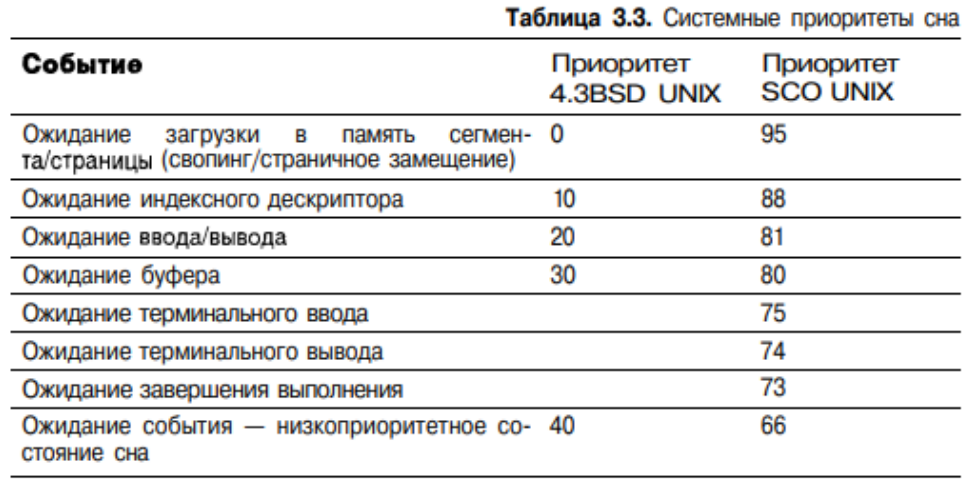
\includegraphics[width=0.90\linewidth]{resources/sleep.png}
    \caption{Системные приоритеты сна}
    \label{fig:rob}
\end{figure}

Каждую секунду ядро системы инициализирует отложенный вызов процедуры
\texttt{schedcpu}, которая уменьшает значение \texttt{p\_pri} каждого процесса
исходя из фактора <<полураспада>> (в системе 4.3BSD считается по
формуле~\ref{eq:ref1})

\begin{equation}
    \label{eq:ref1}
    \mathtt{decay} = \frac{2 \cdot \mathtt{load\_average}}{2 \cdot
    \mathtt{load\_average} + 1}.
\end{equation}

Здесь \texttt{load\_average}~--- это среднее количество процессов, находящихся
в состоянии готовности к выполнению, за последнюю секунду.

Также процедура \texttt{schedcpu} пересчитывает приоритеты для режима задачи
всех процессов по формуле~\ref{eq:ref2}:

\begin{equation}
    \label{eq:ref2}
    \mathtt{p\_usrpri} = \mathtt{PUSER} + \frac{\mathtt{p\_cpu}}{2} + 2 \cdot
    \mathtt{p\_nice}.
\end{equation}

Здесь \texttt{PUSER}~--- базовый приоритет в режиме задачи, равный 50.

Таким образом, если процесс в последний раз использовал большое количество
процессорного времени, то его \texttt{р\_срu} будет увеличен \( \Rightarrow \)
рост значения \texttt{p\_usrpri} \( \Rightarrow \) понижение приоритета. Чем
дольше процесс простаивает в очереди на выполнение, тем больше фактор
полураспада уменьшает его \texttt{р\_срu} \( \Rightarrow \) повышение его
приоритета. Такая схема предотвращает бесконечное откладывание
низкоприоритетных процессов. Применение данной схемы предпочтительно процессам,
осуществляющим много операций ввода-вывода, в противоположность процессам,
производящим много вычислений. То есть динамический пересчет приоритетов
процессов в режиме задачи позволяет избежать бесконечного откладывания.

\section{Вывод}

Операционные системы семейств Unix и Windows являются системами разделения
времени с динамическими приоритетами и вытеснением, поэтому функции обработчика
прерывания от системного таймера в этих системах выполняют схожие задачи:
\begin{itemize}
    \item декремент кванта текущего процесса в UNIX и декремент текущего потока
        в Windows;
    \item инициализация отложенных действий, которые относятся к работе
        планировщика (например, пересчет приоритетов);
    \item инкремент различных счетчиков времени.
\end{itemize}

Пересчет динамических приоритетов осуществляется только для пользовательских
процессов для того, чтобы избежать бесконечного откладывания.

\end{document}
